\documentclass[mask,man]{apa6}

\usepackage{amssymb,amsmath}
\usepackage{ifxetex,ifluatex}
\usepackage{fixltx2e} % provides \textsubscript
\ifnum 0\ifxetex 1\fi\ifluatex 1\fi=0 % if pdftex
  \usepackage[T1]{fontenc}
  \usepackage[utf8]{inputenc}
\else % if luatex or xelatex
  \ifxetex
    \usepackage{mathspec}
    \usepackage{xltxtra,xunicode}
  \else
    \usepackage{fontspec}
  \fi
  \defaultfontfeatures{Mapping=tex-text,Scale=MatchLowercase}
  \newcommand{\euro}{€}
\fi
% use upquote if available, for straight quotes in verbatim environments
\IfFileExists{upquote.sty}{\usepackage{upquote}}{}
% use microtype if available
\IfFileExists{microtype.sty}{\usepackage{microtype}}{}

% Table formatting
\usepackage{longtable, booktabs}
\usepackage{lscape}
% \usepackage[counterclockwise]{rotating}   % Landscape page setup for large tables
\usepackage{multirow}		% Table styling
\usepackage{tabularx}		% Control Column width
\usepackage[flushleft]{threeparttable}	% Allows for three part tables with a specified notes section
\usepackage{threeparttablex}            % Lets threeparttable work with longtable

% Create new environments so endfloat can handle them
% \newenvironment{ltable}
%   {\begin{landscape}\begin{center}\begin{threeparttable}}
%   {\end{threeparttable}\end{center}\end{landscape}}

\newenvironment{lltable}
  {\begin{landscape}\begin{center}\begin{ThreePartTable}}
  {\end{ThreePartTable}\end{center}\end{landscape}}

  \usepackage{ifthen} % Only add declarations when endfloat package is loaded
  \ifthenelse{\equal{\string man}{\string man}}{%
   \DeclareDelayedFloatFlavor{ThreePartTable}{table} % Make endfloat play with longtable
   % \DeclareDelayedFloatFlavor{ltable}{table} % Make endfloat play with lscape
   \DeclareDelayedFloatFlavor{lltable}{table} % Make endfloat play with lscape & longtable
  }{}%



% The following enables adjusting longtable caption width to table width
% Solution found at http://golatex.de/longtable-mit-caption-so-breit-wie-die-tabelle-t15767.html
\makeatletter
\newcommand\LastLTentrywidth{1em}
\newlength\longtablewidth
\setlength{\longtablewidth}{1in}
\newcommand\getlongtablewidth{%
 \begingroup
  \ifcsname LT@\roman{LT@tables}\endcsname
  \global\longtablewidth=0pt
  \renewcommand\LT@entry[2]{\global\advance\longtablewidth by ##2\relax\gdef\LastLTentrywidth{##2}}%
  \@nameuse{LT@\roman{LT@tables}}%
  \fi
\endgroup}


  \usepackage{graphicx}
  \makeatletter
  \def\maxwidth{\ifdim\Gin@nat@width>\linewidth\linewidth\else\Gin@nat@width\fi}
  \def\maxheight{\ifdim\Gin@nat@height>\textheight\textheight\else\Gin@nat@height\fi}
  \makeatother
  % Scale images if necessary, so that they will not overflow the page
  % margins by default, and it is still possible to overwrite the defaults
  % using explicit options in \includegraphics[width, height, ...]{}
  \setkeys{Gin}{width=\maxwidth,height=\maxheight,keepaspectratio}
\ifxetex
  \usepackage[setpagesize=false, % page size defined by xetex
              unicode=false, % unicode breaks when used with xetex
              xetex]{hyperref}
\else
  \usepackage[unicode=true]{hyperref}
\fi
\hypersetup{breaklinks=true,
            pdfauthor={},
            pdftitle={The role of salience in young children's processing of ad-hoc implicatures},
            colorlinks=true,
            citecolor=blue,
            urlcolor=blue,
            linkcolor=black,
            pdfborder={0 0 0}}
\urlstyle{same}  % don't use monospace font for urls

\setlength{\parindent}{0pt}
%\setlength{\parskip}{0pt plus 0pt minus 0pt}

\setlength{\emergencystretch}{3em}  % prevent overfull lines


% Manuscript styling
\captionsetup{font=singlespacing,justification=justified}
\usepackage{csquotes}
\usepackage{upgreek}

 % Line numbering
  \usepackage{lineno}
  \linenumbers


\usepackage{tikz} % Variable definition to generate author note

% fix for \tightlist problem in pandoc 1.14
\providecommand{\tightlist}{%
  \setlength{\itemsep}{0pt}\setlength{\parskip}{0pt}}

% Essential manuscript parts
  \title{The role of salience in young children's processing of ad-hoc
implicatures}

  \shorttitle{Children's ad-hoc implicature processing}


  \author{Erica J. Yoon\textsuperscript{1}~\& Michael C. Frank\textsuperscript{1}}

  % \def\affdep{{"", ""}}%
  % \def\affcity{{"", ""}}%

  \affiliation{
    \vspace{0.5cm}
          \textsuperscript{1} Stanford University  }

  \authornote{
    We would like to acknowledge Asher Kaye, Stephanie Hsiang, and
    Jacqueline Quirke for their assistance in data collection, and thank the
    staff and families at Children's Discovery Museum of San Jose and Bing
    Nursery School. All data, analysis code, and experiment files and links
    and their preregistration are available at
    \url{https://github.com/ejyoon/simpimp_rs}. This work was supported by a
    Postgraduate Doctoral Fellowship provided to EJY by Natural Sciences and
    Engineering Research Council of Canada, NSF \#1456077, and Jacobs
    Advanced Research Fellowship to MCF.
    
    Correspondence concerning this article should be addressed to Erica J.
    Yoon, Department of Psychology, Jordan Hall, 450 Serra Mall (Bldg. 420),
    Stanford, CA, 94305. E-mail:
    \href{mailto:ejyoon@stanford.edu}{\nolinkurl{ejyoon@stanford.edu}}
  }


  \abstract{Language comprehension often requires making \emph{implicatures}. For
example, inferring that ``I ate some of the cookies'' implicates the
speaker ate some \emph{but not all} (scalar implicatures); and ``I ate
the chocolate-chip cookies'' where there are both chocolate chip cookies
and raisin cookies in the context implicates that the speaker ate the
chocolate chip, but \emph{not both the chocolate chip and raisin
cookies} (ad-hoc implicatures). Children's ability to make scalar
implicatures develops around age five, with ad-hoc implicatures emerging
somewhat earlier. In the current work, using a time-sensitive tablet
paradigm, we examined developmental gains in children's ad-hoc
implicature processing, and found evidence for successful pragmatic
inferences by children as young as 3 years in a supportive context and
substantial developmental gains in inference computation from 2 to 5
years. We also tested whether one cause of younger children
(2-year-olds)'s consistent failure to make pragmatic inferences is their
difficulty in inhibiting an alternative interpretation that is more
salient than the target meaning (the \emph{salience hypothesis}). Our
findings supported this hypothesis: Younger children's failures with
pragmatic inferences were related to effects of the salience mismatch
between possible interpretations.}
  \keywords{Pragmatics; cognitive development; language processing; implicature;
tablet \\

    \indent Word count: 9136
  }





\begin{document}

\maketitle

\setcounter{secnumdepth}{0}



Language comprehension in context often requires inferring an intended
meaning that goes beyond the literal semantics of what a speaker says.
Consider a speaker who asserts that:

\begin{enumerate}
\def\labelenumi{(\arabic{enumi})}
\tightlist
\item
  I ate some of the cookies.
\end{enumerate}

\noindent A reasonable listener could assume from this sentence that the
speaker ate some \emph{but not all of the cookies}. Inferences like this
one, known as \emph{implicatures}, are commonplace in conversation and
provide one important tool for speakers to use language flexibly. They
also are related to a broader set of pragmatic phenomena like
underspecification (Levinson, 2000) and politeness (P. Brown \&
Levinson, 1987).

How does the ability to make pragmatic inferences develop in childhood?
A general finding is that implicature follows a relatively delayed
trajectory, with even school-aged children sometimes struggling with
implicature tasks (Noveck, 2001). A rich literature has explored both
these developmental changes and possible hypotheses about the sources of
difficulty for children (e.g., Barner, Brooks, \& Bale, 2011; Papafragou
\& Musolino, 2003; Stiller, Goodman, \& Frank, 2015). These
investigations are important because they shed light on developmental
changes in children's ability to comprehend language in context more
broadly, as well as the processing challenges posed by pragmatic
language comprehension.

In the current paper, we investigate the developmental trajectory of the
processing of one specific type of implicatures, \emph{ad-hoc
implicatures}, which tend to be easier for young children than other
implicatures that rely on more sophisticated linguistic knowledge
(Horowitz, Schneider, \& Frank, 2018; Papafragou \& Musolino, 2003;
Stiller et al., 2015). In addition, we test a specific proposal for why
young children might find even these inferences challenging, namely that
the inferential target is typically less salient than the distractor. In
the remainder of the Introduction, before describing our own work we
first introduce pragmatic implicature in more depth, then review
developmental evidence on implicature.

\subsection{Pragmatic Implicature}\label{pragmatic-implicature}

In Grice (1975)'s classic account of pragmatic inference, conversation
is a cooperative act. Speakers choose utterances such that the listener
can understand the intended message, and listeners in turn interpret
these utterances with the assumption of the speaker's cooperativeness in
mind. The listener then expects a cooperative speaker to have produced
an utterance that is truthful, informative, relevant, and concise,
relative to the the present conversational needs. Based on these
expectations, the listener can make inferences that go beyond the
literal meanings of the speaker's words. The non-literal interpretations
computed through these inferential processes are called pragmatic
implicatures.

A concrete example of such an implicature follows from sentence (1),
which implicates that the speaker ate some \emph{but not all of the
cookies}. This kind of inference is often referred to as a \emph{scalar
implicature} because it relies on the fact that \enquote{all of the
cookies} entails \enquote{some of the cookies} as part of a lexical
scale (Horn, 1972). In contrast, another kind of implicature,
\emph{ad-hoc implicature}, is context-based. Uttering:

\begin{enumerate}
\def\labelenumi{(\arabic{enumi})}
\setcounter{enumi}{1}
\tightlist
\item
  I ate the chocolate chip cookies.
\end{enumerate}

\noindent in a context where two kinds of cookies -- chocolate chip and
raisin -- are available, implicates that the speaker ate the chocolate
chip \emph{but not both the chocolate chip cookies and raisin
cookies}.\footnote{Grice (1975) calls these implicatures generalized
  (scalar) vs.~particularized (ad-hoc), but we use a theory-neutral
  designation here.} In this case, the context sets up a contrast
between the proposition offered (\enquote{ate the chocolate chip
cookies}) and a stronger set of alternatives (\enquote{ate {[}all/both
the chocolate chip and the raisin{]} the cookies}) that is determined by
the context (and hence is \enquote{ad hoc} in the sense of being
constructed in this particular situation).

Implicatures like these have been an important case study for pragmatics
more broadly. Notably, different accounts of pragmatic reasoning analyze
even the simple examples above in different ways. In the classic Gricean
analysis (as elaborated by Levinson, 1983), the speaker utters \emph{p}
(\enquote{some of the cookies}), which implicates \emph{q} (\enquote{not
all of the cookies}) in the following way. (A) The speaker is presumed
to be cooperative and observing Grice's maxims. (B) To maintain this
assumption, the listener must assume that \emph{q} is true; otherwise a
maxim will be violated. (In this case the maxim is informativeness,
since saying \enquote{some of the cookies} if \enquote{all of the
cookies} were true would be underinformative). (C) The speaker is
presumed to believe that it is mutually known by both parties that the
listener can work out \emph{q}.

This analysis -- though influential -- is in fact just one proposal
among many, and likely does not map onto either the mental computations
carried out by listeners or the specific issues that lead to
developmental differences in implicature ability. Both classic theories
of communication (e.g., Sperber \& Wilson, 1995) and more recent
probabilistic models of pragmatic inference (e.g., Frank \& Goodman,
2012; see Goodman \& Frank, 2016 for review) describe the processes that
language users use to compute such implicatures in different ways. For
example, Chierchia, Fox, and Spector (2012) give an account of
implicature as a specific, grammaticalized operation that involves
enriching the meaning of \emph{p} with the negation of all stronger
alternatives within a specified alternative set. In contrast, on the
probabilistic view, implicatures arise naturally as part of the process
of cooperative reasoning by rational agents.

Our goal here is not to distinguish between these different formalisms;
instead, we are interested in understanding the processing of
implicature in childhood. Despite that, it is useful to review the
probabilistic view as it helps guide some of our predictions below. We
consider sentence (2), following the analysis given in Goodman and Frank
(2016). Under the rational speech act (RSA) model, there is a space of
meanings (e.g., ATE(chocolate chip \& raisin), ATE(chocolate chip),
etc.), each of which may have some prior probability of being correct.
There is also a space of utterances (e.g., \enquote{I ate the chocolate
chip cookies,} \enquote{I ate the cookies}), each of which is either
literally consistent or inconsistent with each meaning. Given a
particular utterance, a listener can reason probabilistically about the
speaker's intended meaning in making this utterance. He can do this by
considering that the speaker is a Bayesian agent who chose the
appropriate utterance for her intended meaning. He reasons about the
speaker making her own choice by considering a listener who is also a
Bayesian agent reasoning in this same way. This definition is endlessly
recursive, however. In practice, the recursion can be grounded by a
speaker considering a \enquote{literal listener,} who interprets
utterances according to their literal truth value (for further formal
details, see Goodman \& Frank, 2016).

In the specific case of (2), the listener's reasoning can be glossed as
\enquote{if the speaker had wanted to say she ate \enquote{all of the
cookies}, she could have said just \enquote{cookies}; but she didn't,
she said something more specific: \enquote{chocolate chip}; thus she
probably intended me to recover the meaning ATE(chocolate chip).} Notice
that this reasoning, when explained verbally, actually approximates the
standard Gricean logic (though with some differences). Of course, one
benefit of the RSA formalism is that probabilities can be put to each of
these inferences and so the strength of the interpretive judgment can be
predicted (Frank \& Goodman, 2012). On the other hand, the RSA-style
reasoning differs from other implicature accounts that stress the
intentionality of the speaker to convey a stronger meaning through the
expression of a weaker meaning (e.g., Bach, 1999) and that hence grant a
privileged status to implicatures specifically. In contrast, RSA treats
implicature like other general cases of contextual disambiguation.

\subsection{The Development of Pragmatic
Implicature}\label{the-development-of-pragmatic-implicature}

A rich psycholinguistic literature has measured adults' processing of
implicatures relative to literal interpretations and has found that
adults robustly compute implicatures in a range of contexts, though
their processing time can vary depending on the context (Bott, Bailey,
\& Grodner, 2012; Breheny, Ferguson, \& Katsos, 2013; Grodner, Klein,
Carbary, \& Tanenhaus, 2010; Huang \& Snedeker, 2018). How does the
ability to make implicatures develop? Since implicature computation is
an important indicator of broader pragmatic understanding, many studies
have tested children's abilities on a variety of implicatures.

Children tend to have the most difficulty with scalar implicatures
relying on quantifiers, modals, and other functional elements. For
example, in Papafragou and Musolino (2003)'s study, a puppet saw three
out of three horses jump over a fence, and described the scene
infelicitously by saying \enquote{Some of the horses jumped over the
fence.} Adults tend to reject this infelicitous statement, whereas
5-year-old children mostly accept it, suggesting that children failed to
compute the relevant scalar implicature (though see Katsos \& Bishop,
2011, for an alternative explanation). Besides struggling with
\emph{some} vs. \emph{all} (Huang \& Snedeker, 2009; Hurewitz,
Papafragou, Gleitman, \& Gelman, 2006; Noveck, 2001), children in the
same age range have consistently failed to compute implicatures
involving scalar contrasts, including \emph{a} vs. \emph{some} (Barner,
Chow, \& Yang, 2009), \emph{might} vs. \emph{must} (Noveck, 2001), and
\emph{or} vs. \emph{and} (Chierchia, Crain, Guasti, Gualmini, \& Meroni,
2001).

While children struggle on many scalar implicature tasks, they tend to
be more successful at computing ad-hoc implicatures (which depend on
context, rather than lexical scales). One potential difficulty in a
typical scalar implicature task is the need to generate relevant
alternatives to a given scalar term. For children to hear \enquote{some
of the horses jumped over the fence} and derive the implicature
\enquote{some \emph{but not all},} they must first realize that
\enquote{all} is the relevant alternative to \enquote{some.} Barner et
al. (2011) argued that children's failures in scalar implicature tasks
are due to their lack of ability to generate the alternative to negate
spontaneously upon hearing the term offered. Barner et al. (2011)'s
claim predicts that children's implicature computation should improve
when they can access the relevant alternatives. Consistent with this
claim, children can be primed with relevant scalar alternatives, leading
to enhanced implicature performance (Skordos \& Papafragou, 2016).
Furthermore, children show substantially improved implicature
computation in ad-hoc implicature tasks -- which provided access to
relevant alternatives in context -- compared to scalar implicature tasks
(Horowitz et al., 2018; Katsos \& Bishop, 2011; Papafragou \& Tantalou,
2004; Stiller et al., 2015).

For example, Stiller et al. (2015) showed 2.5- to 5-year-old children
three different faces: a face with no item; a face with only glasses;
and a face with glasses and a top-hat, and asked children to choose one
of the three faces as the referent in a puppet's statement, \enquote{My
friend has glasses.} In this task, the alternative referent (face with
glasses and hat) was visible in the context, and thus access to the
alternative terms (\enquote{glasses and hat}) was made easier. In
general, we assume that the standard route for referring to these visual
properties of the context will be by naming them. The design intention
in this study for using simple nouns like \enquote{hat} was therefore to
make it obvious what the linguistic alternatives would be by virtue of
the highly accessible names for stimuli. Children as young as 3.5 years
chose the face with only glasses as the referent, suggesting that they
successfully computed the implicature that the puppet's friend has
\enquote{glasses but not both glasses and hat.} Similarly, in one study
that tested both scalar and ad-hoc implicature computation, 4-year-olds
successfully made ad-hoc implicatures, but performed poorly on scalar
implicatures using the same stimuli (Horowitz et al., 2018).

Despite older children's success, children below 3 years of age appear
to struggle with even simple ad-hoc implicatures. Even in the ad-hoc
paradigm described above (Stiller et al., 2015), 2.5- and 3-year-olds
still did not make the implicature-consistent choice at above-chance
levels. Does this finding imply that young toddlers lack pragmatic
understanding, specifically an awareness of the need for informativeness
in cooperative communication? On the contrary, children are sensitive to
informativeness in communication: From age two onward, when they are
asked to produce referring expressions, children appear to recognize the
level of referential ambiguity of their own expressions and attempt to
provide more information through speech and gestures in more ambiguous
situations (e.g., instead of ``the boy,'' saying ``the boy with the
dog''; or naming an object while pointing in cases where the point alone
is not precise enough; Matthews, Butcher, Lieven, \& Tomasello, 2012;
O'Neill \& Topolovec, 2001). Hence, a lack of sensitivity to the need
for communicative informativeness does not seem to be the problem for
toddlers' implicature processing. So what causes toddlers' failures in
these easier ad-hoc implicature tasks specifically?

\subsection{The Current Study}\label{the-current-study}

One potential explanation for younger children's struggle with ad-hoc
implicatures is the mismatch in salience between potential
interpretations. This explanation is inspired by the RSA framework
described above, in the sense that this salience mismatch would be
manifest in the pragmatic computation as a higher prior probability of a
particular referent. For example, in Stiller et al. (2015)'s study, a
target referent (e.g., face with glasses only) had fewer features than
its alternative distractor to be rejected (e.g., face with glasses and
hat). The distractor, which had a greater number of nameable features,
was more salient both perceptually and conceptually, likely drawing
children's attention more strongly than the target. Under the RSA
framework -- and very likely under other pragmatic theories, though
perhaps with a less clearly specified prediction -- such a mismatch in
prior probabilities would lead to a weaker pragmatic inference.

The mismatch between stimulus salience (prior probability) and the
target of the pragmatic inference may be particularly difficult
developmentally. From a mechanistic perspective, a task with this kind
of competition between targets may be especially challenging to children
because their executive function is not yet fully developed (Davidson,
Amso, Anderson, \& Diamond, 2006; Diamond \& Taylor, 1996), and
specifically their ability to inhibit responses to salient targets (but
see Discussion for further consideration of whether children's failures
should be attributed to their inhibitory control abilities per se).

Such an issue might be important outside of the specific case of ad-hoc
implicature and referent-selection tasks. For example, referent
selection tasks may be representative of analogous problems in
naturalistic language comprehension for children, in which the goal is
often to figure out what referent a speaker is talking about or how to
connect a new word to a new referent (in the case of word learning;
Frank \& Goodman, 2014). And in such situations, there is a body of
evidence suggesting that referent salience does in fact influence
children's attention (Hollich et al., 2000; Yurovsky \& Frank, 2017).

Further, under RSA analysis given above there is no fundamental
difference between referent selection tasks and other implicature
comprehension tasks. Thus, the asymmetry between correct but weaker
target meaning and incorrect but more salient or higher prior
probability distractor meaning is present in other types of implicatures
too, though less obviously so. For example, scalar implicature is
typically described as rejecting the term that yields the
\enquote{stronger} propositional meaning (e.g., ate \enquote{all} of the
cookies) and adding its negation to the \enquote{weaker} proposition
(e.g., \enquote{some but not all} of the cookies). Computing a
forced-choice scalar implicature thus also requires avoiding the
stronger meaning, which typically describes a larger set size. Although
the referents in such tasks are not always pictured visually
side-by-side, they are in at least some paradigms (e.g., Huang \&
Snedeker, 2009). At least in these cases -- and perhaps more generally
-- the stronger alternative could reasonably be viewed as being more
salient or higher prior probability. And, as above, when prior
probabilities (whether induced by perceptual factors like salience or
emerging from other sources) conflict with pragmatic inferences, the
resulting comprehension situation may be especially difficult for
children.

For all of these reasons, in our current work, we were interested in
exploring the issue of distractor salience and how it played out in the
development of implicature processing for children. For our experiment,
we adopted a referent selection method, in which participants were asked
to select a referent among a set of candidates. As mentioned earlier,
referent selection paradigms have shown evidence of successful
implicature computation in youngest children to date (Horowitz et al.,
2018; Stiller et al., 2015), and are analogous to one important aspect
of of language comprehension in naturalistic language environments,
namely identifying a speaker's intended referent (On the other hand,
because such paradigms can be solved by RSA-style agents that are not
specifically focused on implicating a particular meaning, we are
cautious below in interpreting success as evidence of implicature per
se. For convenience, however we still, refer to these as ad-hoc
implicature \emph{tasks}).

This setup allowed us to create a systematic manipulation of the stimuli
in our referent selection method. Under the RSA model, the more
alternative utterances there are to refer to a particular referent, the
less likely any one of them is. Thus, adding more features to the
distractor referent in the referent selection task should make it even
less likely as the referent of any particular one. For example, in the
faces case used by Stiller et al. (2015), if the target is a face with
glasses, then a face with a hat, glasses, and a mustache (three
features) should be a \emph{worse} distractor referent for
\enquote{glasses} than a face with just a hat and glasses (two
features). Frank and Goodman (2014) tested this prediction with adults
in a word-learning case and found quantitative support for the idea that
the number of features was related to the strength of pragmatic
judgments.

The interesting thing about this manipulation, however, is that it might
very well have an \emph{opposite} effect on young children because of
the referent salience explanation given above. While a distractor with
more features should create a stronger pragmatic inference, it should
also be more salient to young children, leading to a higher prior
probability and worse performance. Thus, in our current experiment we
predicted that young children would struggle differentially in the case
there were more features on the distractor, while older children would
find this case no more difficult and perhaps even easier.

We stress that, although our manipulation was inspired by the RSA model,
it does not depend on that model. As touched on above, there are a
variety of different accounts that try to explain exactly what pragmatic
inference children are making in ad-hoc implicature tasks. In the
Stiller et al. (2015) example, \enquote{my friend has glasses} can
implicate \enquote{my friend has glasses \emph{but no hat}} based on the
immediate context. A slightly different interpretation could be:
\enquote{\ldots{}glasses \emph{but no other distinguishing features},}
however (exhaustivity implicature; Groenendijk \& Stokhof, 1985). For
the purposes of the current work, we cannot differentiate between these
proposals -- as long as an account incorporated prior information in
some fashion, it would likely make a similar prediction. Thus, our goal
is not to make a test of a particular implicature account, but rather to
test the idea that referent salience (instantiated as prior probability
in the RSA model) affects children's implicature behavior.

In our experiment, we implemented the referent selection task using a
tablet paradigm. This methodological change allowed us to examine
children's reaction times for selecting the target referent along with
their specific selection (Frank, Sugarman, Horowitz, Lewis, \& Yurovsky,
2016). Compared to previous studies, we also reduced the number of
potential referents in context to further simplify the task. In Stiller
et al. (2015)'s paradigm, there were three potential referents in the
context (face with no item, face with only glasses, face with glasses
and hat); in our current paradigm, we presented two instead of three
potential referents (e.g.~plate with a carrot and plate with a carrot
and a banana) to minimize cognitive load for the younger children in our
task.

We present data here from two independent samples: The first planned
sample of children across four age groups (2-, 3-, 4-, and 5-year-olds)
initially showed a pattern consistent with the salience hypothesis,
where children were more accurate for trials with lower salience
contrasts than for trials with higher salience contrasts. This effect
was relatively small, however, and our analysis plan was not
prespecified, leading us to worry about the possibility that analytic
flexibility might have led us to overestimate our effect (e.g., Simmons,
Nelson, \& Simonsohn, 2011). We thus collected a second, fully
preregistered sample of children across the three youngest groups (2-,
3- and 4-year-olds) to replicate this initial finding and make a
stronger test of the hypothesis.

\section{Methods}\label{methods}

We report how we determined our sample size, all data exclusions (if
any), all manipulations, and all measures in the study.

\begin{table}[tbp]
\begin{center}
\begin{threeparttable}
\caption{\label{tab:participantsummarytab}Demographic information of participants in the original and replication samples.}
\begin{tabular}{llllll}
\toprule
Sample & \multicolumn{1}{c}{Age bin} & \multicolumn{1}{c}{Number of participants} & \multicolumn{1}{c}{Mean (years)} & \multicolumn{1}{c}{SD (years)} & \multicolumn{1}{c}{\% Girls}\\
\midrule
original & 2 & 25 & 2.51 & 0.31 & 72.00\\
original & 3 & 29 & 3.54 & 0.28 & 55.20\\
original & 4 & 26 & 4.45 & 0.29 & 34.60\\
original & 5 & 19 & 5.30 & 0.23 & 57.90\\
replication & 2 & 25 & 2.66 & 0.27 & 56.00\\
replication & 3 & 30 & 3.47 & 0.28 & 56.70\\
replication & 4 & 25 & 4.39 & 0.29 & 40.00\\
\bottomrule
\end{tabular}
\end{threeparttable}
\end{center}
\end{table}

\subsection{Participants}\label{participants}

In the original sample, either parents and their children visiting
Children's Discovery Museum (San Jose, CA), or children in a local
nursery school were invited to participate in a tablet study, and a
total of 120 children were recruited. Participants were excluded from
the sample for the following reasons: age other than 2 to 5 years
(\emph{n} = 3); parent-reported English exposure less than our
prespecified criterion of 75\% (\emph{n} = 5); parental interference
(\emph{n} = 2); and noncompliance or difficulty with the experimental
procedure (\emph{n} = 9). After excluding participants who completed
fewer than the prespecified number of 10 trials (\emph{n} = 2), the
final sample consisted of 99 children (see Table
\ref{tab:participantsummarytab}).

In the replication sample, a total of 116 children were recruited, all
at Children's Discovery Museum in San Jose. Reasons for exclusions were:
age other than 2 to 4 years (\emph{n} = 11); parent-reported English
exposure less than our prespecified criterion of 75\% (\emph{n} = 15);
parental interference (\emph{n} = 3); noncompliance or difficulty with
the experimental procedure (\emph{n} = 3); and technical error (\emph{n}
= 4). The final sample consisted of 80 children (no participant was
excluded for completing fewer than 10 trials). It should be noted that
we deviated from our preregistered sample since we did not recruit
5-year-olds, as we saw 4-year-olds already performing at ceiling and
thus considered 4-year-olds to suffice as the oldest group.

\subsection{Stimuli and Design}\label{stimuli-and-design}

\begin{figure}
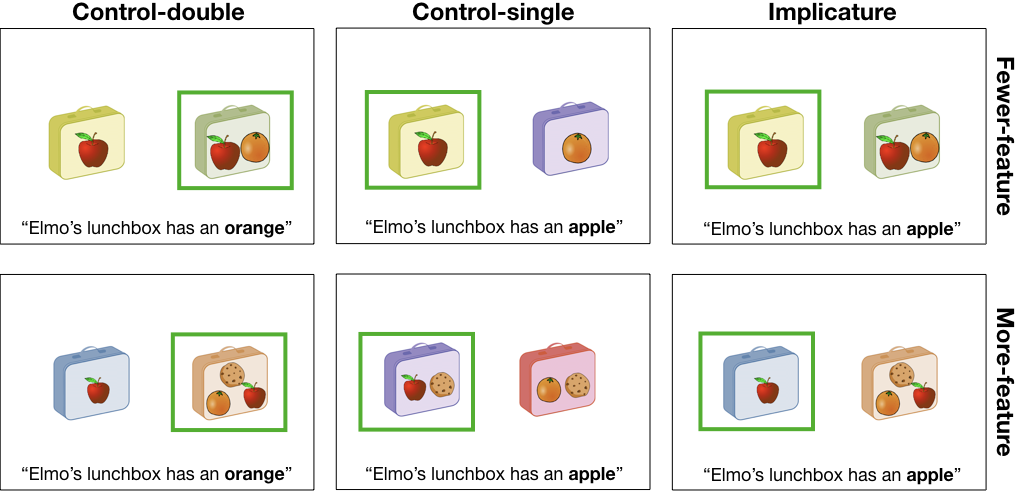
\includegraphics[width=5.98in]{figs/stimuli} \caption{Trial types. Green box indicates the target referent for each trial given the utterance at the bottom.}\label{fig:stimuli}
\end{figure}

On each trial, participants saw two images: a target and distractor,
which could either be an item with a single feature (e.g.~a lunchbox
with only an apple), or an item with double features (e.g., a lunchbox
with an apple and an orange). In each trial, a pre-recorded voice said a
sentence (e.g., \enquote{Look at these lunchboxes. Elmo's lunchbox has
an apple.}). After participants chose the object that was being referred
to, a green box appeared around the chosen object to show that the
choice had been made. For each trial, we recorded the participant's
accuracy, or whether he or she selected the correct target referent, and
reaction time, or time spent between naming of the referent
(\enquote{\ldots{}an \emph{apple}}) and the participant's referent
selection.

There were three types of test trials (shown at the top of each panel in
Figure \ref{fig:stimuli}). In \emph{implicature} trials, the target item
had a single feature (e.g., an apple), and the distractor item had two
or three features (see below for the manipulation of number of features)
-- one that was in common with the target (e.g., an apple) and the other
feature(s) that was/were unique (e.g., an orange). The test sentence
named the feature that was common to the target and distractor. Thus, if
participants understood that \enquote{Elmo's lunchbox has an apple}
implicates \enquote{Elmo's lunchbox has an apple \emph{but not an
orange}} in the given context, it was predicted that they would choose
the target more often than the distractor; otherwise, if they did not
make implicatures, they would choose the two at equal rates (or even
choose the distractor more often depending on the degree of saliency
contrast -- see below).

There were two additional trial types, with semantically unambiguous
targets: \emph{Control-double} trials looked identical to implicature
trials, but the target and distractor were switched, such that the
double-feature item was the target and the single-feature item was the
distractor, and the test sentence named the unique feature on the
target. \emph{Control-single} trials presented two items that each had a
unique single feature, and either could be the target. Children saw 4
implicature, 4 control-double, and 8 control-single trials; adults saw 6
implicature, 6 control-double, and 12 control-single trials.

Each trial type was further divided by the number of features present on
the target and distractor (shown on the right side of Figure
\ref{fig:stimuli}): Within implicature trials, \emph{fewer-feature}
(2-vs-1) trials presented two features (an apple and an orange) on the
distractor and one feature (an apple) on the target, whereas
\emph{more-feature} (3-vs-1) trials presented three features (an apple,
an orange, and a cookie) on the distractor and one feature on the
target; Within control-double trials, \emph{fewer-feature} (2-vs-1)
trials presented two features (an apple and an orange) on the target and
one feature (an apple) on the distractor, whereas \emph{more-feature}
(3-vs-1) trials presented three features (an apple, an orange, and a
cookie) on the distractor and one feature on the target; Lastly, within
control-single trials, \emph{fewer-feature} (1-vs-1) trials presented
one feature each on the distractor and the target, whereas
\emph{more-feature} (2-vs-2) trials presented two features each on the
distractor and on the target.

We hypothesized that older children would choose the target more often
in the more-feature implicature trials than the fewer-feature
implicature trials because implicatures are strengthened more in
more-feature trials -- \enquote{Elmo's lunchbox has an apple} is more
likely to mean \enquote{apple only} given an orange AND cookie on the
alternative referent, thus more things that could have been named but
were not. On the contrary, younger children were predicted to choose the
target less often in the more-feature trials than the fewer-feature
trials because the distractor is more salient in the fewer-feature
trials, while still being consistent with the literal meaning.

There were six sets of item and feature types, and the features were
named with nouns found on the MacArthur-Bates Communicative Development
Inventory word list (Fenson et al., 1994). Two orders of the test trials
were created, such that trial types and item types were counterbalanced
and trial order was pseudo-randomized across the two orders.

\subsection{Procedure}\label{procedure}

An experimenter introduced children to the task as a game on a tablet.
Then they completed two practice trials, where they were asked to select
an obvious, unambiguous referent (e.g., \enquote{cow} as opposed to
\enquote{rabbit}), followed by 16 test trials.

\subsection{Data analysis}\label{data-analysis}

We used R (Version 3.4.3; R Core Team, 2017) and the R-packages
\emph{bindrcpp} (Version 0.2.2; Müller, 2017a), \emph{brms} (Version
2.0.1; Bürkner, 2017), \emph{dplyr} (Version 0.8.0.1; Wickham, Francois,
Henry, \& Müller, 2017), \emph{forcats} (Version 0.2.0; Wickham, 2017a),
\emph{ggplot2} (Version 3.0.0; Wickham, 2009), \emph{ggthemes} (Version
3.4.0; Arnold, 2017), \emph{here} (Version 0.1; Müller, 2017b),
\emph{langcog} (Version 0.1.9001; Braginsky, Yurovsky, \& Frank, n.d.),
\emph{lme4} (Version 1.1.15; D. Bates, Mächler, Bolker, \& Walker,
2015), \emph{Matrix} (Version 1.2.12; D. Bates \& Maechler, 2017),
\emph{papaja} (Version 0.1.0.9655; Aust \& Barth, 2017), \emph{purrr}
(Version 0.2.5; Henry \& Wickham, 2017), \emph{Rcpp} (Eddelbuettel \&
Balamuta, 2017; Version 1.0.1; Eddelbuettel \& François, 2011),
\emph{readr} (Version 1.1.1; Wickham, Hester, \& Francois, 2017),
\emph{stringr} (Version 1.3.1; Wickham, 2017b), \emph{tibble} (Version
2.1.1; Müller \& Wickham, 2017), \emph{tidyr} (Version 0.7.2; Wickham \&
Henry, 2017), \emph{tidyverse} (Version 1.2.1; Wickham, 2017c), and
\emph{xtable} (Version 1.8.2; Dahl, 2016) for all our analyses.

\section{Results}\label{results}

We were interested in children's processing of implicatures in
comparison to unambiguous utterances, and developmental gains across
ages. We used two different measures: (1) accuracy and (2) reaction time
for choosing the correct referent. For each measure, we asked: (a) do
children show developmental gains in selection of the target referent?
And (b) does children's performance vary depending on salience contrast?
That is, when there are a relatively greater number of features on the
distractor, do children have more difficulty and are they slower in
choosing the correct referent?

As per our standard operating procedures, we removed trials in which the
log of reaction time was more than 3 standard deviations above or below
the mean (upper bound: 13.57 seconds; lower bound: 0.49 second;
percentage of data excluded: 1.66 \%). Throughout this section, we used
Bayesian linear mixed-effects models (\texttt{brms} package in R;
Bürkner, 2017) using crossed random effects of participant and item with
the maximal random effects structure supported by the design (Barr,
Levy, Scheepers, \& Tily, 2013; A. Gelman \& Hill, 2006). Age is plotted
in year bins, but was analyzed as a continuous variable, scaled and
centered, in our statistical model.

\begin{figure}
\centering
\includegraphics{simpimp_paper_files/figure-latex/accuracy-1.pdf}
\caption{\label{fig:accuracy}Proportion of 2- to 5-year-old children
selecting the target in the original and replication samples (rows) in
different trial types (columns). Data are binned into 6-month age groups
for visualization purposes (all analyses are conducted on continuous
data). Lines are loess smoothing functions. Solid lines represent trials
in which there were fewer features present (2-vs-1 for control-double
and implicature, 1-vs-1 for control-single) and dashed lines represent
trials with more features (3-vs-1 for control-double and implicature,
2-vs-2 for control-single). Error bars are 95\% confidence intervals,
and are placed at the mean of the age bin and offset slightly to avoid
overplotting. Dotted line represents a conservative chance level at
50\%.}
\end{figure}

\subsection{Accuracy}\label{accuracy}

\begin{table}[tbp]
\begin{center}
\begin{threeparttable}
\caption{\label{tab:brmaccSample1}Predictor mean estimates with standard deviation and 95\% credible interval information for a Bayesian linear mixed-effects model predicting accurate selection of target for the original sample.}
\begin{tabular}{lllll}
\toprule
Predictor & \multicolumn{1}{c}{Mean} & \multicolumn{1}{c}{SD} & \multicolumn{1}{c}{95\% CI-Lower} & \multicolumn{1}{c}{95\% CI-Upper}\\
\midrule
Intercept & 4.00 & 0.51 & 3.08 & 5.10\\
Age & 1.58 & 0.36 & 0.93 & 2.33\\
Control-double & -0.39 & 0.67 & -1.68 & 0.99\\
Implicature & -2.23 & 0.68 & -3.64 & -0.95\\
More features & 0.12 & 0.59 & -1.08 & 1.31\\
Control-double * Age & -0.57 & 0.44 & -1.45 & 0.32\\
Implicature * Age & -0.39 & 0.43 & -1.27 & 0.44\\
More features * Age & -0.36 & 0.41 & -1.17 & 0.43\\
Control-double * More features & -0.42 & 0.73 & -1.82 & 1.03\\
Implicature * More features & 0.12 & 0.76 & -1.30 & 1.72\\
Control-double * Age * More features & 0.44 & 0.57 & -0.69 & 1.56\\
Implicature * Age * More features & 0.78 & 0.53 & -0.24 & 1.84\\
\bottomrule
\end{tabular}
\end{threeparttable}
\end{center}
\end{table}

\begin{table}[tbp]
\begin{center}
\begin{threeparttable}
\caption{\label{tab:brmaccSample2}Predictor mean estimates with standard deviation and 95\% credible interval information for a Bayesian linear mixed-effects model predicting accurate selection of target for the replication sample.}
\begin{tabular}{lllll}
\toprule
Predictor & \multicolumn{1}{c}{Mean} & \multicolumn{1}{c}{SD} & \multicolumn{1}{c}{95\% CI-Lower} & \multicolumn{1}{c}{95\% CI-Upper}\\
\midrule
Intercept & 6.63 & 1.30 & 4.50 & 9.47\\
Age & 3.52 & 0.94 & 1.95 & 5.60\\
Control-double & -0.35 & 1.44 & -2.95 & 2.70\\
Implicature & -3.98 & 1.43 & -6.94 & -1.32\\
More features & -1.32 & 1.35 & -4.17 & 1.13\\
Control-double * Age & -1.04 & 1.07 & -3.09 & 1.17\\
Implicature * Age & -2.20 & 0.90 & -4.12 & -0.63\\
More features * Age & -1.29 & 0.95 & -3.27 & 0.48\\
Control-double * More features & 0.11 & 1.47 & -2.83 & 2.97\\
Implicature * More features & -0.04 & 1.48 & -2.95 & 2.87\\
Control-double * Age * More features & 0.98 & 1.25 & -1.49 & 3.41\\
Implicature * Age * More features & 1.62 & 0.97 & -0.15 & 3.61\\
\bottomrule
\end{tabular}
\end{threeparttable}
\end{center}
\end{table}

\begin{table}[tbp]
\begin{center}
\begin{threeparttable}
\caption{\label{tab:brmacc}Predictor mean estimates with standard deviation and 95\% credible interval information for a Bayesian linear mixed-effects model predicting accurate selection of target in both the original and replication samples.}
\begin{tabular}{lllll}
\toprule
Predictor & \multicolumn{1}{c}{Mean} & \multicolumn{1}{c}{SD} & \multicolumn{1}{c}{95\% CI-Lower} & \multicolumn{1}{c}{95\% CI-Upper}\\
\midrule
Intercept & 4.09 & 0.47 & 3.21 & 5.08\\
Sample & 0.69 & 0.26 & 0.20 & 1.20\\
Age & 1.81 & 0.31 & 1.23 & 2.45\\
Control-double & -0.42 & 0.58 & -1.57 & 0.73\\
Implicature & -2.55 & 0.67 & -3.86 & -1.26\\
More features & -0.15 & 0.55 & -1.30 & 0.90\\
Control-double * Age & -0.72 & 0.37 & -1.46 & 0.01\\
Implicature * Age & -0.67 & 0.35 & -1.36 & 0.00\\
More features * Age & -0.47 & 0.35 & -1.16 & 0.20\\
Control-double * More features & -0.29 & 0.61 & -1.44 & 0.93\\
Implicature * More features & 0.00 & 0.63 & -1.23 & 1.26\\
Control-double * Age * More features & 0.51 & 0.49 & -0.45 & 1.47\\
Implicature * Age * More features & 0.89 & 0.43 & 0.07 & 1.74\\
\bottomrule
\end{tabular}
\end{threeparttable}
\end{center}
\end{table}

The analysis of the accuracy rate (Figure \ref{fig:accuracy}) showed
that children across all ages were able to identify the target in
control trials, indicating that, as expected, they can readily compute
unambiguous meanings. In implicature trials, 4- and 5-year-olds'
performances were nearly at ceiling, replicating the previous results
(Horowitz et al., 2018; Stiller et al., 2015). In our paradigm, even
3-year-olds chose the inferential target above chance\footnote{Because
  our task is a two-alternative forced choice, we define chance to be
  50\% across all trials. This baseline is a standard comparison that
  reflects the possibility that a child was completely inattentive to
  the task and chose completely at random. This baseline is more
  conservative than a salience-based baseline, which would likely
  suggest that the correct (inferentially-consistent) target would be
  chosen less than 50\% of the time (e.g., the \enquote{mumble}
  condition in Stiller et al., 2015).} (original sample: \(t\)(57) =
6.65, \(p\) \textless{} 0.001; replication sample: \(t\)(59) = 5.71,
\(p\) \textless{} 0.001). On the other hand, 2-year-olds' performance in
implicature trials did not differ from chance overall, but their
performance varied depending on the number of features present. In
3-vs-1 trials (i.e., with a relatively greater number of features on the
distractor), 2-year-olds did not choose the correct target referent, and
even tended to choose the distractor somewhat more often numerically
(original sample: \(t\)(23) = -1.42, \(p\) = 0.17; replication sample:
\(t\)(24) = -0.72, \(p\) = 0.48). However, In 2-vs-1 trials (with fewer
features on the distractor), 2-year-olds tended to choose the target
more often than the distractor. This difference was numerically present
in both samples and statistically significant in one (original sample:
\(t\)(24) = 0.24, \(p\) = 0.81; replication sample: \(t\)(24) = 2.57,
\(p\) = 0.02). By 4 years, this difference in accuracy rate between
2-vs-1 and 3-vs-1 trials was not present.

Bayesian linear mixed models predicting accuracy based on age, trial
type and number of features (salience contrast; more-feature
vs.~fewer-feature) were conducted separately on the original sample and
replication sample (Table \ref{tab:brmaccSample1} and Table
\ref{tab:brmaccSample2}). Both models showed a main effect of age and a
main effect of implicature trials, which indicated that children
performed more poorly on implicature trials than control trials, while
their overall performance on all trial types improved with age. In
addition, the model for the replication sample showed a two-way negative
interaction between age and implicature trials, which suggested that
improvement with age for implicature trials was lower compared to
control trials for the replication sample.

We ran an exploratory Bayesian linear mixed-effects model on combined
datasets from the original and replication sample, predicting accuracy
based on age, trial type and number of features, which showed a
three-way positive interaction of age, implicature trials, and number of
features (Table \ref{tab:brmacc}). Unlike control trials, in which
children's performances did not differ by salience contrast, implicature
trials showed lower accuracy in 3-vs-1 than 2-vs-1 trials in younger
children, but not in older children. Thus, this result supports our
hypothesis that the salience contrast between conditions led to greater
difficulty with the implicature task for for younger children.

\subsection{Reaction time}\label{reaction-time}

\begin{figure}
\centering
\includegraphics{simpimp_paper_files/figure-latex/rt-1.pdf}
\caption{\label{fig:rt}Reaction time to select the correct target referent.
Conventions are identical to Figure 2.}
\end{figure}

\begin{table}[tbp]
\begin{center}
\begin{threeparttable}
\caption{\label{tab:brmrtSample1}Predictor mean estimates with standard deviation and 95\% credible interval information for a Bayesian linear mixed-effects model predicting log reaction time to select the target for the original sample.}
\begin{tabular}{lllll}
\toprule
Predictor & \multicolumn{1}{c}{Mean} & \multicolumn{1}{c}{SD} & \multicolumn{1}{c}{95\% CI-Lower} & \multicolumn{1}{c}{95\% CI-Upper}\\
\midrule
Intercept & 7.70 & 0.04 & 7.61 & 7.78\\
Age & -0.21 & 0.03 & -0.27 & -0.15\\
Control-double & 0.04 & 0.08 & -0.11 & 0.17\\
Implicature & 0.17 & 0.08 & 0.01 & 0.32\\
More features & 0.10 & 0.06 & -0.03 & 0.22\\
Control-double * Age & -0.04 & 0.04 & -0.12 & 0.04\\
Implicature * Age & 0.10 & 0.04 & 0.02 & 0.17\\
More features * Age & 0.02 & 0.03 & -0.04 & 0.08\\
Control-double * More features & 0.10 & 0.07 & -0.03 & 0.23\\
Implicature * More features & 0.03 & 0.08 & -0.13 & 0.19\\
Control-double * Age * More features & 0.02 & 0.05 & -0.08 & 0.12\\
Implicature * Age * More features & -0.07 & 0.05 & -0.17 & 0.03\\
\bottomrule
\end{tabular}
\end{threeparttable}
\end{center}
\end{table}

\begin{table}[tbp]
\begin{center}
\begin{threeparttable}
\caption{\label{tab:brmrtSample2}Predictor mean estimates with standard deviation and 95\% credible interval information for a Bayesian linear mixed-effects model predicting log reaction time to select the target for the replication sample.}
\begin{tabular}{lllll}
\toprule
Predictor & \multicolumn{1}{c}{Mean} & \multicolumn{1}{c}{SD} & \multicolumn{1}{c}{95\% CI-Lower} & \multicolumn{1}{c}{95\% CI-Upper}\\
\midrule
Intercept & 7.81 & 0.04 & 7.74 & 7.88\\
Age & -0.21 & 0.03 & -0.27 & -0.15\\
Control-double & 0.01 & 0.07 & -0.15 & 0.14\\
Implicature & 0.17 & 0.09 & -0.02 & 0.34\\
More features & 0.10 & 0.06 & -0.02 & 0.22\\
Control-double * Age & 0.02 & 0.03 & -0.04 & 0.08\\
Implicature * Age & 0.11 & 0.03 & 0.04 & 0.17\\
More features * Age & 0.05 & 0.03 & 0.00 & 0.10\\
Control-double * More features & 0.12 & 0.06 & 0.01 & 0.24\\
Implicature * More features & -0.10 & 0.07 & -0.24 & 0.05\\
Control-double * Age * More features & -0.02 & 0.04 & -0.11 & 0.06\\
Implicature * Age * More features & -0.07 & 0.04 & -0.16 & 0.01\\
\bottomrule
\end{tabular}
\end{threeparttable}
\end{center}
\end{table}

\begin{table}[tbp]
\begin{center}
\begin{threeparttable}
\caption{\label{tab:brmrt}Predictor mean estimates with standard deviation and 95\% credible interval information for a Bayesian linear mixed-effects model predicting log reaction time to select the target in both the original and replication samples.}
\begin{tabular}{lllll}
\toprule
Predictor & \multicolumn{1}{c}{Mean} & \multicolumn{1}{c}{SD} & \multicolumn{1}{c}{95\% CI-Lower} & \multicolumn{1}{c}{95\% CI-Upper}\\
\midrule
Intercept & 7.73 & 0.03 & 7.67 & 7.79\\
Sample & 0.03 & 0.04 & -0.04 & 0.10\\
Age & -0.21 & 0.02 & -0.25 & -0.17\\
Control-double & 0.03 & 0.07 & -0.11 & 0.15\\
Implicature & 0.16 & 0.10 & -0.02 & 0.33\\
More features & 0.10 & 0.06 & -0.01 & 0.22\\
Control-double * Age & -0.01 & 0.02 & -0.06 & 0.04\\
Implicature * Age & 0.10 & 0.03 & 0.05 & 0.15\\
More features * Age & 0.03 & 0.02 & -0.01 & 0.07\\
Control-double * More features & 0.11 & 0.05 & 0.01 & 0.20\\
Implicature * More features & -0.02 & 0.06 & -0.14 & 0.11\\
Control-double * Age * More features & 0.00 & 0.03 & -0.07 & 0.07\\
Implicature * Age * More features & -0.06 & 0.04 & -0.13 & 0.01\\
\bottomrule
\end{tabular}
\end{threeparttable}
\end{center}
\end{table}

With increasing age, children computed both implicatures and unambiguous
meanings and identified the target faster (Figure \ref{fig:rt}).
Bayesian linear mixed-effects models predicting reaction time based on
age, trial type and number of features were conducted separately in the
original sample and replication sample, and showed a positive two-way
interaction between age and implicature trial (Table
\ref{tab:brmrtSample1} and Table \ref{tab:brmrtSample2}), indicating
that reaction time on implicature trials did not improve with age as
much as the speed of processing unambiguous meanings. This interaction
was also shown in an exploratory Bayesian linear mixed-effects model on
the combined datasets with both samples (Table \ref{tab:brmrt}).
Together with the accuracy finding, this result suggests that though
children become proficient at determining the \emph{correct} target
referents for ad-hoc implicatures by 5 years, implicature processing
develops relatively more slowly.

In two of the three models (the model on the replication sample only and
the model on both datasets together), we also observed a positive
two-way interaction between control-double trials and number of
features, indicating that children took longer to identify the target in
control-double trials with more features than in control-single trials
with more features.

There was no interaction between inference trials and number of
features, or between inference trial, age and number of features,
however. Why would this be? We did not have a pre-specified hypothesis
regarding this pattern of data, but we speculate that once a feature is
named (e.g., Elmo's lunchbox has an apple), it is relatively easier to
find the feature in an inferential target image than in the distractor
image. The target feature is by itself in the target referent, whereas
it is grouped with with other features in the distractor. Thus, the
inference trials may allow easy perceptual access to the target feature
but also competition with the overall perceptual salience of the
distractor. These factors might cancel one another out and lead to
undifferentiated reaction times and hence the lack of reaction time
interactions. The potential advantage of identifying a feature when it
is by itself is only speculative, however, and should be examined
further in future work.

\subsection{Reliability}\label{reliability}

\begin{table}[tbp]
\begin{center}
\begin{threeparttable}
\caption{\label{tab:alphaTable}Standardized reliability coefficients (Cronbach's $\alpha$) for accuracy (acc) and reaction time (RT) by age group, along with the mean number of trials for each.}
\begin{tabular}{llll}
\toprule
Age bin & \multicolumn{1}{c}{$M$ trials} & \multicolumn{1}{c}{$\alpha_{acc}$} & \multicolumn{1}{c}{$\alpha_{rt}$}\\
\midrule
2 & 11.40 & 0.70 & 0.65\\
3 & 11.68 & 0.80 & 0.80\\
4 & 11.88 & 0.48 & 0.84\\
5 & 11.79 & 0.21 & 0.28\\
\bottomrule
\end{tabular}
\end{threeparttable}
\end{center}
\end{table}

As specified in our preregistered protocol, we measured Cronbach's
alpha, a statistic that determines the internal consistency of
experimental items (Santos, 1999). We selected the 12 control trials and
computed a reliability coefficient for each age group, for both RTs and
accuracies. Reliabilities are shown in Table \ref{tab:alphaTable}.
Reliabilities for 2-, 3- year olds and adults were reasonable (
\textgreater{} .7). reliabilities for accuracy were lower amongst 4- and
5-year olds due to ceiling effects; for 4-year-olds, reaction time still
showed high reliability. For 5-year-olds, neither RT nor accuracy were
reliable, likely indicating that this paradigm was simply too easy for
them (replicating results from Frank et al., 2016).

\section{Discussion}\label{discussion}

In our experiment, we confirmed 3- to 5-year-old children's successes on
pragmatic inferences, and saw substantial developmental gains in their
accuracy and speed. 4- and 5-year-old children successfully computed
pragmatic inferences and identified the inferential targets, consistent
with previous findings. We found evidence of successful pragmatic
inferences even in 3-year-olds. Further, between 2 and 5 years, there
was a clear improvement in processing skills with increasing age, such
that correct referent identification was more accurate and faster across
both control and implicature trials. Thus, these findings add to the
existing literature to attest to children's growing proficiency in
pragmatic processing.

We also investigated the salience hypothesis, namely that one cause of
young children's struggle with pragmatic inferences stems from their
difficulty to inhibit choosing the more salient distractor. In earlier
work, there was some numerical suggestion of 2-year-olds' preference for
the more salient but pragmatically incorrect distractor (Stiller et al.,
2015). Inspired by this pattern and following the predictions of the RSA
model of pragmatic inference, we predicted that increasing the salience
of this distractor would result in decreased performance for younger
children while increasing performance for older children. The first part
of this prediction was clearly supported in our data, with younger
children performing worse when the distractor was more salient, with
more mixed support for the second part.

In particular, although we observed numerical hints of a gain in
accuracy for older children in one sample, we did not see a consistent
facilitation effect due to our manipulation. We suspect this finding is
due to a ceiling effect: Referent selection via ad-hoc implicature is
relatively trivial for four-year-olds (see also Horowitz et al., 2018).
However, we saw a possible age-related advantage of pragmatic
strengthening in the speed of computation: Whereas younger children
tended to be slower in trials with a greater number of features for both
unambiguous and inferential meanings, older children began to close the
gap and become faster to compute implicatures given increased distractor
saliency.

Our findings here support the idea that salience-related competition
plays a role in young children's difficulties with ad-hoc implicature
tasks. Our salience account is most manifest in the kind of simple
referent selection tasks we used here. Despite this, following the
general mapping of perceptual salience to prior probabilities in the RSA
framework more broadly, we speculate that the account may apply more
broadly to implicature computation beyond the scope of these tasks. Any
pragmatic implicature requires an asymmetry in the \enquote{strength} of
the alternatives. In ad-hoc referent-selection contexts, the stronger
(more salient) alternative is the item with more features. In scalar
implicatures, the implicature that you ate \emph{some but not all of the
cookies} is only possible because there is a stronger alternative
(\enquote{all}). It remains an open empirical question whether the
salience mismatch account -- perhaps relabeled as a prior probability
mismatch -- might explain some aspects of children's difficulty with
these other cases of implicatures as well.

The salience hypothesis we tested here relates to broader methodological
issues in experiments for young children with both visual and verbal
alternative responses. One example of such a bias is the tendency of
2-year-olds to show a bias toward \enquote{yes} compared to \enquote{no}
in answering questions. This bias disappears with age (Fritzley \& Lee,
2003), and there is some evidence that it is related to children's
verbal ability and inhibitory control (Moriguchi, Okanda, \& Itakura,
2008). In general, as work on pragmatic inference begins to examine
younger children's abilities, it is important to take into consideration
a range of cognitive factors in task design.

Following this line of reasoning, one further potential application of
our account is to word learning contexts, where children's learning of a
novel word is facilitated when the target referent is more (not less)
salient than its alternative. For example, Frank and Goodman (2014) used
an analogous pragmatic inference paradigm in a word learning context:
Participants heard a novel label (e.g., \enquote{a dinosaur with a
\emph{dax}}) used to describe an object with two features (a dinosaur
with a hat and a bandanna) in the presence of another dinosaur that had
one but not the other of the features (a dinosaur with a hat only). 3-
and 4-year-olds performed quite well in mapping the novel label to the
unique feature, even though in many respects this task should be more,
not less, difficult than ad-hoc implicature. One reason for this success
might be that the novel label was being mapped to the more, rather than
less, salient object.

Similarly, in classic \enquote{mutual exclusivity} paradigms (Markman \&
Wachtel, 1988), by around 18 months, participants succeed in mapping a
novel label to a novel object (Halberda, 2003). While the mechanisms
underlying this empirical phenomenon are complex, it is well-established
that the salience of the novel target is an important factor in
children's success (see Markman, Wasow, \& Hansen, 2003 for discussion).
Overall, evidence for children's pragmatic word learning emerges earlier
than implicature computation: Children succeed in these tasks
substantially at earlier ages than even in our simplified implicature
paradigm. We might speculate that one reason for this asymmetry is
because implicature tasks require selecting the \emph{less} salient
alternative while word learning tasks typically ask participants to
select a \emph{more} salient alternative.

Our findings help in the construction of a comprehensive developmental
account of processing of implicatures, and pragmatic inferences in
general. In the samples that have been studied in this literature, by 2
years of age, children begin to be aware that informativeness is
important to communication. By 3 to 4 years, the ability to inhibit
these salient targets is more developed, and they start to compute
ad-hoc implicatures when relevant alternatives to the speaker's words
are provided in context. Scalar implicature performance develops more
slowly, however, as children's ability to access the relevant
inferential alternatives is only beginning to emerge in the period from
4 to 6 (Barner et al., 2011; Horowitz et al., 2018; Skordos \&
Papafragou, 2016); their performance during these ages is highly
variable and dependent on the nature of the context and its pragmatic
demands (Papafragou \& Tantalou, 2004).

As illustrated by this timeline, the salience hypothesis we tested is
not mutually exclusive with other accounts of children's difficulties in
implicature. For example, the \enquote{alternatives hypothesis} (Barner
et al., 2011) is independently supported by a variety of experiments
(Horowitz et al., 2018; Skordos \& Papafragou, 2016). Indeed, both the
salience and alternatives hypotheses are likely true and likely
contribute to children's difficulty with implicatures to different
degrees in different tasks and at different ages.

One important challenge for this viewpoint is the nature of the ability
that children use to overcome the pull of the salient alternative. One
possible naive mapping for the ability would be to the broader construct
of executive function, which undergoes substantial developmental changes
during this period (Davidson et al., 2006; Diamond \& Taylor, 1996). But
executive function is a multi-faceted construct (Miyake et al., 2000),
and the particular components that would be expected to predict visual
(and perhaps conceptual) disengagement with a particular referent is
unclear. Our own studies attempting to probe individual difference
correlations between executive function and implicature ability in
development have not been successful (e.g., Horowitz et al., 2018;
Nordmeyer, Yoon, \& Frank, 2016). Thus, a target for future work is to
better characterize the particular cognitive changes that relate to the
developmental effects we have observed here.

There are several further limitations of our work here. First, our
salience manipulation involved manipulation of the number of features
present on an item, which might have caused a potential confound between
salience and processing time. For example, children's greater looking to
the distractor (and thus greater processing time) might have been caused
by a real desire to acquire more information, rather than the mere
perceptual salience of the distractors. Second, as noted in the
Introduction, our study does not differentiate between different
theoretical proposals about how pragmatic inference is being computed in
the current task. However, we believe that we are addressing development
of implicatures in general, with a caveat that our definition of
implicatures does pertain to broader inferential reasoning between
speakers and listeners, rather than having a special status or mechanism
as assumed under particular formalisms. Third, as with nearly all work
in the literature on implicature processing, we address the performance
of only relatively high socioeconomic status children in a Western
context. In our ongoing work we address the generalizability of our task
to other developmental contexts (Fortier, Kellier, Fernández Flecha, \&
Frank, in prep).

In sum, our work shows evidence that from at least 3 years, children are
able to compute ad-hoc implicatures, and that younger children's
failures with implicatures on an referent-choosing task are confounded
by the salience mismatch between possible referents. This pattern is
consistent with a broader generalization, namely that tasks that have
typically been used to look at children's implicature processing have a
variety of extraneous processing demands, which may explain why it has
been difficult to see children's underlying pragmatic abilities in such
paradigms. Thus, our work demonstrates the importance of using a range
of methods to measure children's pragmatic processing.

\newpage

\section{References}\label{references}

\setlength{\parindent}{-0.5in} \setlength{\leftskip}{0.5in}

\hypertarget{refs}{}
\hypertarget{ref-R-ggthemes}{}
Arnold, J. B. (2017). \emph{Ggthemes: Extra themes, scales and geoms for
'ggplot2'}. Retrieved from
\url{https://CRAN.R-project.org/package=ggthemes}

\hypertarget{ref-R-papaja}{}
Aust, F., \& Barth, M. (2017). \emph{papaja: Create APA manuscripts with
R Markdown}. Retrieved from \url{https://github.com/crsh/papaja}

\hypertarget{ref-bach1999}{}
Bach, K. (1999). The myth of conventional implicature. \emph{Linguistics
and Philosophy}, \emph{22}(4), 327--366.

\hypertarget{ref-barner2011}{}
Barner, D., Brooks, N., \& Bale, A. (2011). Accessing the unsaid: The
role of scalar alternatives in children's pragmatic inference.
\emph{Cognition}, \emph{118}(1), 84--93.
doi:\href{https://doi.org/10.1016/j.cognition.2010.10.010}{10.1016/j.cognition.2010.10.010}

\hypertarget{ref-barner2009}{}
Barner, D., Chow, K., \& Yang, S.-J. (2009). Finding one's meaning: A
test of the relation between quantifiers and integers in language
development. \emph{Cognitive Psychology}, \emph{58}(2), 195--219.
doi:\href{https://doi.org/10.1016/j.cogpsych.2008.07.001}{10.1016/j.cogpsych.2008.07.001}

\hypertarget{ref-barr2013random}{}
Barr, D. J., Levy, R., Scheepers, C., \& Tily, H. J. (2013). Random
effects structure for confirmatory hypothesis testing: Keep it maximal.
\emph{Journal of Memory and Language}, \emph{68}(3), 255--278.

\hypertarget{ref-R-Matrix}{}
Bates, D., \& Maechler, M. (2017). \emph{Matrix: Sparse and dense matrix
classes and methods}. Retrieved from
\url{https://CRAN.R-project.org/package=Matrix}

\hypertarget{ref-R-lme4}{}
Bates, D., Mächler, M., Bolker, B., \& Walker, S. (2015). Fitting linear
mixed-effects models using lme4. \emph{Journal of Statistical Software},
\emph{67}(1), 1--48.
doi:\href{https://doi.org/10.18637/jss.v067.i01}{10.18637/jss.v067.i01}

\hypertarget{ref-bott2012}{}
Bott, L., Bailey, T. M., \& Grodner, D. J. (2012). Distinguishing speed
from accuracy in scalar implicatures. \emph{Journal of Memory and
Language}, \emph{66}(1), 123--142.
doi:\href{https://doi.org/10.1016/j.jml.2011.09.005}{10.1016/j.jml.2011.09.005}

\hypertarget{ref-R-langcog}{}
Braginsky, M., Yurovsky, D., \& Frank, M. C. (n.d.). \emph{Langcog:
Language and cognition lab things}. Retrieved from
\url{http://github.com/langcog/langcog}

\hypertarget{ref-breheny2013}{}
Breheny, R., Ferguson, H. J., \& Katsos, N. (2013). Taking the epistemic
step: Toward a model of on-line access to conversational implicatures.
\emph{Cognition}, \emph{126}(3), 423--440.
doi:\href{https://doi.org/10.1016/j.cognition.2012.11.012}{10.1016/j.cognition.2012.11.012}

\hypertarget{ref-brown1987}{}
Brown, P., \& Levinson, S. C. (1987). \emph{Politeness: Some universals
in language usage} (Vol. 4). Cambridge University Press.

\hypertarget{ref-R-brms}{}
Bürkner, P.-C. (2017). brms: An R package for bayesian multilevel models
using Stan. \emph{Journal of Statistical Software}, \emph{80}(1), 1--28.
doi:\href{https://doi.org/10.18637/jss.v080.i01}{10.18637/jss.v080.i01}

\hypertarget{ref-chierchia2001}{}
Chierchia, G., Crain, S., Guasti, M. T., Gualmini, A., \& Meroni, L.
(2001). The acquisition of disjunction: Evidence for a grammatical view
of scalar implicatures. In \emph{Proceedings of BUCLD 25} (Vol. 157, p.
168).

\hypertarget{ref-chierchia2012}{}
Chierchia, G., Fox, D., \& Spector, B. (2012). Scalar implicature as a
grammatical phenomenon. In Maienborn, von Heusinger, \& Portner (Eds.),
\emph{Semantics: An international handbook of natural language meaning}
(Vol. 3). New York: Mouton de Gruyter.

\hypertarget{ref-R-xtable}{}
Dahl, D. B. (2016). \emph{Xtable: Export tables to latex or html}.
Retrieved from \url{https://CRAN.R-project.org/package=xtable}

\hypertarget{ref-davidson2006}{}
Davidson, M. C., Amso, D., Anderson, L. C., \& Diamond, A. (2006).
Development of cognitive control and executive functions from 4 to 13
years: Evidence from manipulations of memory, inhibition, and task
switching. \emph{Neuropsychologia}, \emph{44}(11), 2037--2078.
doi:\href{https://doi.org/10.1016/j.neuropsychologia.2006.02.006}{10.1016/j.neuropsychologia.2006.02.006}

\hypertarget{ref-diamond1996}{}
Diamond, A., \& Taylor, C. (1996). Development of an aspect of executive
control: Development of the abilities to remember what I said and to
``do as I say, not as I do''. \emph{Developmental Psychobiology},
\emph{29}, 315--334.
doi:\href{https://doi.org/10.1002/(SICI)1098-2302(199605)29:4/\%3C315::AID-DEV2/\%3E3.3.CO;2-C}{10.1002/(SICI)1098-2302(199605)29:4\textbackslash{}\%3C315::AID-DEV2\textbackslash{}\%3E3.3.CO;2-C}

\hypertarget{ref-R-Rcpp_b}{}
Eddelbuettel, D., \& Balamuta, J. J. (2017). Extending extitR with
extitC++: A Brief Introduction to extitRcpp. \emph{PeerJ Preprints},
\emph{5}, e3188v1.
doi:\href{https://doi.org/10.7287/peerj.preprints.3188v1}{10.7287/peerj.preprints.3188v1}

\hypertarget{ref-R-Rcpp_a}{}
Eddelbuettel, D., \& François, R. (2011). Rcpp: Seamless R and C++
integration. \emph{Journal of Statistical Software}, \emph{40}(8),
1--18.
doi:\href{https://doi.org/10.18637/jss.v040.i08}{10.18637/jss.v040.i08}

\hypertarget{ref-fenson1994}{}
Fenson, L., Dale, P. S., Reznick, J. S., Bates, E., Thal, D. J.,
Pethick, S. J., \ldots{} Stiles, J. (1994). Variability in early
communicative development. \emph{Monographs of the Society for Research
in Child Development}, i--185.
doi:\href{https://doi.org/10.2307/1166093}{10.2307/1166093}

\hypertarget{ref-fortierunderrev}{}
Fortier, M., Kellier, D., Fernández Flecha, M., \& Frank, M. C. (in
prep). Ad-hoc pragmatic implicatures among shipibo-konibo children in
the peruvian amazon.
doi:\href{https://doi.org/10.17605/OSF.IO/X7AD9}{10.17605/OSF.IO/X7AD9}

\hypertarget{ref-frank2012}{}
Frank, M. C., \& Goodman, N. D. (2012). Predicting pragmatic reasoning
in language games. \emph{Science}, \emph{336}(6084), 998--998.
doi:\href{https://doi.org/10.1016/j.cogpsych.2014.08.002}{10.1016/j.cogpsych.2014.08.002}

\hypertarget{ref-frank2014}{}
Frank, M. C., \& Goodman, N. D. (2014). Inferring word meanings by
assuming that speakers are informative. \emph{Cognitive Psychology},
\emph{75}, 80--96.
doi:\href{https://doi.org/10.1016/j.cogpsych.2014.08.002}{10.1016/j.cogpsych.2014.08.002}

\hypertarget{ref-frank2016}{}
Frank, M. C., Sugarman, E., Horowitz, A. C., Lewis, M. L., \& Yurovsky,
D. (2016). Using tablets to collect data from young children.
\emph{Journal of Cognition and Development}, \emph{17}, 1--17.
doi:\href{https://doi.org/10.1080/15248372.2015.1061528}{10.1080/15248372.2015.1061528}

\hypertarget{ref-fritzley2003young}{}
Fritzley, H. V., \& Lee, K. (2003). Do young children always say yes to
yes--no questions? A metadevelopmental study of the affirmation bias.
\emph{Child Development}, \emph{74}(5), 1297--1313.

\hypertarget{ref-gelman2006data}{}
Gelman, A., \& Hill, J. (2006). \emph{Data analysis using regression and
multilevel/hierarchical models}. Cambridge university press.

\hypertarget{ref-goodman2016}{}
Goodman, N. D., \& Frank, M. C. (2016). Pragmatic language
interpretation as probabilistic inference. \emph{Trends in Cognitive
Sciences}, \emph{20}(11), 818--829.

\hypertarget{ref-grice1975logic}{}
Grice, H. P. (1975). Logic and conversation. \emph{Syntax and
Semantics}, \emph{3}, 41--58.

\hypertarget{ref-grodner2010}{}
Grodner, D. J., Klein, N. M., Carbary, K. M., \& Tanenhaus, M. K.
(2010). ?Some,? And possibly all, scalar inferences are not delayed:
Evidence for immediate pragmatic enrichment. \emph{Cognition},
\emph{116}(1), 42--55.

\hypertarget{ref-groenendijk1985semantics}{}
Groenendijk, J., \& Stokhof, M. (1985). On the semantics of questions
and the pragmatics of answers. \emph{Semantics: Critical Concepts in
Linguistics}, \emph{288}.

\hypertarget{ref-halberda2003development}{}
Halberda, J. (2003). The development of a word-learning strategy.
\emph{Cognition}, \emph{87}(1), B23--B34.

\hypertarget{ref-R-purrr}{}
Henry, L., \& Wickham, H. (2017). \emph{Purrr: Functional programming
tools}. Retrieved from \url{https://CRAN.R-project.org/package=purrr}

\hypertarget{ref-hollich2000}{}
Hollich, G. J., Hirsh-Pasek, K., Golinkoff, R. M., Brand, R. J., Brown,
E., Chung, H. L., \ldots{} Bloom, L. (2000). Breaking the language
barrier: An emergentist coalition model for the origins of word
learning. \emph{Monographs of the Society for Research in Child
Development}, i--135.
doi:\href{https://doi.org/10.1111/1540-5834.00090}{10.1111/1540-5834.00090}

\hypertarget{ref-horn1972}{}
Horn, L. R. (1972). \emph{On the semantic properties of logical
operators in english} (PhD thesis). University of California, Los
Angeles.

\hypertarget{ref-horowitz2018}{}
Horowitz, A. C., Schneider, R. M., \& Frank, M. C. (2018). The trouble
with quantifiers: Exploring children's deficits in scalar implicature.
\emph{Child Development}, \emph{89}(6), e572--e593.

\hypertarget{ref-huang2009b}{}
Huang, Y. T., \& Snedeker, J. (2009). Semantic meaning and pragmatic
interpretation in 5-year-olds: Evidence from real-time spoken language
comprehension. \emph{Developmental Psychology}, \emph{45}(6), 1723.
doi:\href{https://doi.org/10.1037/a0016704}{10.1037/a0016704}

\hypertarget{ref-huang2018}{}
Huang, Y. T., \& Snedeker, J. (2018). Some inferences still take time:
Prosody, predictability, and the speed of scalar implicatures.
\emph{Cognitive Psychology}, \emph{102}, 105--126.

\hypertarget{ref-hurewitz2006}{}
Hurewitz, F., Papafragou, A., Gleitman, L., \& Gelman, R. (2006).
Asymmetries in the acquisition of numbers and quantifiers.
\emph{Language Learning and Development}, \emph{2}(2), 77--96.
doi:\href{https://doi.org/10.1207/s15473341lld0202_1}{10.1207/s15473341lld0202\_1}

\hypertarget{ref-katsos2011}{}
Katsos, N., \& Bishop, D. V. (2011). Pragmatic tolerance: Implications
for the acquisition of informativeness and implicature.
\emph{Cognition}, \emph{120}(1), 67--81.
doi:\href{https://doi.org/10.1016/j.cognition.2011.02.015}{10.1016/j.cognition.2011.02.015}

\hypertarget{ref-levinson1983}{}
Levinson, S. C. (1983). Pragmatics. cambridge textbooks in linguistics.
\emph{Cambridge/New York}.

\hypertarget{ref-levinson2000}{}
Levinson, S. C. (2000). \emph{Presumptive meanings: The theory of
generalized conversational implicature}. MIT press.

\hypertarget{ref-markman1988children}{}
Markman, E. M., \& Wachtel, G. F. (1988). Children's use of mutual
exclusivity to constrain the meanings of words. \emph{Cognitive
Psychology}, \emph{20}(2), 121--157.

\hypertarget{ref-markman2003use}{}
Markman, E. M., Wasow, J. L., \& Hansen, M. B. (2003). Use of the mutual
exclusivity assumption by young word learners. \emph{Cognitive
Psychology}, \emph{47}(3), 241--275.

\hypertarget{ref-matthews2012}{}
Matthews, D., Butcher, J., Lieven, E., \& Tomasello, M. (2012). Two-and
four-year-olds learn to adapt referring expressions to context: Effects
of distracters and feedback on referential communication. \emph{Topics
in Cognitive Science}, \emph{4}(2), 184--210.
doi:\href{https://doi.org/10.1111/j.1756-8765.2012.01181.x}{10.1111/j.1756-8765.2012.01181.x}

\hypertarget{ref-miyake2000unity}{}
Miyake, A., Friedman, N. P., Emerson, M. J., Witzki, A. H., Howerter,
A., \& Wager, T. D. (2000). The unity and diversity of executive
functions and their contributions to complex ``frontal lobe'' tasks: A
latent variable analysis. \emph{Cognitive Psychology}, \emph{41}(1),
49--100.

\hypertarget{ref-moriguchi2008young}{}
Moriguchi, Y., Okanda, M., \& Itakura, S. (2008). Young children's yes
bias: How does it relate to verbal ability, inhibitory control, and
theory of mind? \emph{First Language}, \emph{28}(4), 431--442.

\hypertarget{ref-R-bindrcpp}{}
Müller, K. (2017a). \emph{Bindrcpp: An 'rcpp' interface to active
bindings}. Retrieved from
\url{https://CRAN.R-project.org/package=bindrcpp}

\hypertarget{ref-R-here}{}
Müller, K. (2017b). \emph{Here: A simpler way to find your files}.
Retrieved from \url{https://CRAN.R-project.org/package=here}

\hypertarget{ref-R-tibble}{}
Müller, K., \& Wickham, H. (2017). \emph{Tibble: Simple data frames}.
Retrieved from \url{https://CRAN.R-project.org/package=tibble}

\hypertarget{ref-nordmeyer2016}{}
Nordmeyer, A. E., Yoon, E. J., \& Frank, M. C. (2016). Distinguishing
processing difficulties in inhibition, implicature, and negation. In
\emph{Proceedings of the 38th annual meeting of the cognitive science
society}.

\hypertarget{ref-noveck2001}{}
Noveck, I. A. (2001). When children are more logical than adults:
Experimental investigations of scalar implicature. \emph{Cognition},
\emph{78}(2), 165--188.
doi:\href{https://doi.org/10.1016/S0010-0277(00)00114-1}{10.1016/S0010-0277(00)00114-1}

\hypertarget{ref-oneill2001}{}
O'Neill, D. K., \& Topolovec, J. C. (2001). Two-year-old children's
sensitivity to the referential (in) efficacy of their own pointing
gestures. \emph{Journal of Child Language}, \emph{28}(1), 1--28.
doi:\href{https://doi.org/10.1017/S0305000900004566}{10.1017/S0305000900004566}

\hypertarget{ref-papafragou2003}{}
Papafragou, A., \& Musolino, J. (2003). Scalar implicatures: Experiments
at the semantics--pragmatics interface. \emph{Cognition}, \emph{86}(3),
253--282.
doi:\href{https://doi.org/10.1016/S0010-0277(02)00179-8}{10.1016/S0010-0277(02)00179-8}

\hypertarget{ref-papafragou2004}{}
Papafragou, A., \& Tantalou, N. (2004). Children's computation of
implicatures. \emph{Language Acquisition}, \emph{12}(1), 71--82.
doi:\href{https://doi.org/10.1207/s15327817la1201_3}{10.1207/s15327817la1201\_3}

\hypertarget{ref-R-base}{}
R Core Team. (2017). \emph{R: A language and environment for statistical
computing}. Vienna, Austria: R Foundation for Statistical Computing.
Retrieved from \url{https://www.R-project.org/}

\hypertarget{ref-santos1999cronbach}{}
Santos, J. (1999). Cronbach\(\backslash\)'s alpha: A tool for assessing
the reliability of scales. \emph{Journal of Extension}, \emph{37}(2),
1--5.

\hypertarget{ref-simmons2011false}{}
Simmons, J. P., Nelson, L. D., \& Simonsohn, U. (2011). False-positive
psychology: Undisclosed flexibility in data collection and analysis
allows presenting anything as significant. \emph{Psychological Science},
\emph{22}(11), 1359--1366.

\hypertarget{ref-skordos2016}{}
Skordos, D., \& Papafragou, A. (2016). Children's derivation of scalar
implicatures: Alternatives and relevance. \emph{Cognition}, \emph{153},
6--18.
doi:\href{https://doi.org/10.1016/j.cognition.2016.04.006}{10.1016/j.cognition.2016.04.006}

\hypertarget{ref-sperber1986}{}
Sperber, D., \& Wilson, D. (1995). \emph{Relevance: Communication and
cognition}. Oxford: Blackwell.

\hypertarget{ref-stiller2015}{}
Stiller, A., Goodman, N. D., \& Frank, M. C. (2015). Ad-hoc implicature
in preschool children. \emph{Language Learning and Development}.
doi:\href{https://doi.org/10.1080/15475441.2014.927328}{10.1080/15475441.2014.927328}

\hypertarget{ref-R-ggplot2}{}
Wickham, H. (2009). \emph{Ggplot2: Elegant graphics for data analysis}.
Springer-Verlag New York. Retrieved from \url{http://ggplot2.org}

\hypertarget{ref-R-forcats}{}
Wickham, H. (2017a). \emph{Forcats: Tools for working with categorical
variables (factors)}. Retrieved from
\url{https://CRAN.R-project.org/package=forcats}

\hypertarget{ref-R-stringr}{}
Wickham, H. (2017b). \emph{Stringr: Simple, consistent wrappers for
common string operations}. Retrieved from
\url{https://CRAN.R-project.org/package=stringr}

\hypertarget{ref-R-tidyverse}{}
Wickham, H. (2017c). \emph{Tidyverse: Easily install and load the
'tidyverse'}. Retrieved from
\url{https://CRAN.R-project.org/package=tidyverse}

\hypertarget{ref-R-tidyr}{}
Wickham, H., \& Henry, L. (2017). \emph{Tidyr: Easily tidy data with
'spread()' and 'gather()' functions}. Retrieved from
\url{https://CRAN.R-project.org/package=tidyr}

\hypertarget{ref-R-dplyr}{}
Wickham, H., Francois, R., Henry, L., \& Müller, K. (2017). \emph{Dplyr:
A grammar of data manipulation}. Retrieved from
\url{https://CRAN.R-project.org/package=dplyr}

\hypertarget{ref-R-readr}{}
Wickham, H., Hester, J., \& Francois, R. (2017). \emph{Readr: Read
rectangular text data}. Retrieved from
\url{https://CRAN.R-project.org/package=readr}

\hypertarget{ref-yurovsky2017}{}
Yurovsky, D., \& Frank, M. C. (2017). Beyond naive cue combination:
Salience and social cues in early word learning. \emph{Developmental
Science}.
doi:\href{https://doi.org/10.1111/desc.12349}{10.1111/desc.12349}






\end{document}
